% =====================================================================
% StaticKD -- supplementary material for the IEEE Access manuscript (main.tex)
% Compile: pdflatex supplementary && bibtex supplementary && pdflatex supplementary && pdflatex supplementary
% =====================================================================
\documentclass[journal,onecolumn]{IEEEtran}
\usepackage[T1]{fontenc}
\usepackage[utf8]{inputenc}
\usepackage[nocompress]{cite}
\usepackage{amsmath,amssymb}
\usepackage{graphicx}
\usepackage{booktabs}
\usepackage{array}
\usepackage[hyphens]{url}
\usepackage{algorithm}
\usepackage{algpseudocode}
\renewcommand{\thetable}{S\arabic{table}}
\renewcommand{\thefigure}{S\arabic{figure}}
\renewcommand{\thealgorithm}{S\arabic{algorithm}}
\begin{document}
\title{Supplementary Material for ``StaticKD: Distilling a Multilingual IPTC News Topic Classifier into a Static Token-Logit Table for Lightweight CPU Inference''}
\author{Obi~Kastanya, Ananta~Dwi~Prayoga~Alwy, and Dwi~Sunaryono}
\maketitle

The supplementary material contains Algorithm~S1, Tables~S1--S6, Figs.~S1--S7, and additional experimental details cited in the main text.

\begin{algorithm}[!htbp]
\caption{StaticKD Inference for One Article}
\label{alg:infer}
\begin{algorithmic}[1]
\Require article text $d$; tokenizer; table $\bar{T}\in\mathbb{R}^{|V|\times 17}$; bias $\bar{\mathbf{b}}\in\mathbb{R}^{17}$
\State $(t_1,\dots,t_n)\gets$ first 1,024 tokens of tokenize$(d)$, without unknown tokens
\State $\mathbf{z}\gets\frac{1}{n}\sum_{i=1}^{n}\bar{T}_{t_i}+\bar{\mathbf{b}}$ \Comment{look up and average table rows}
\State \Return $\arg\max_{y}\,z_y$ \Comment{one of the 17 IPTC topics}
\end{algorithmic}
\end{algorithm}

\begin{table}[!htbp]
\caption{Hyperparameters of All Models}
\label{tab:hparams}
\centering
\footnotesize
\setlength{\tabcolsep}{3pt}
\resizebox{0.7\textwidth}{!}{%
\begin{tabular}{@{}ll@{}}
\toprule
Component & Value \\
\midrule
\multicolumn{2}{@{}l}{\textit{StaticKD}} \\
\quad initial embedding & potion-multilingual-128M (500,353 $\times$ 256) \\
\quad max. tokens / vector dropout & 1,024 / 0.1 \\
\quad loss, $\tau$ & KL, $\tau=1$ \\
\quad token dropout & 0.2 \\
\quad optimizer embedding / head & SparseAdam $10^{-3}$ / AdamW $3\cdot 10^{-3}$, wd $10^{-4}$ \\
\quad batch, epoch, validation & 64, 6, 3\% of data (selects the epoch) \\
\quad ensemble & mean of 3 seed tables \\
\multicolumn{2}{@{}l}{\textit{fastText}} \\
\quad word tokens (chosen on dev) & dim 300, lr 1.0, 15 epoch \\
\quad subword tokens (chosen on dev) & dim 100, lr 1.0, 15 epoch \\
\quad grid (dev macro-F1) & lr $\{0.1, 0.5, 1.0\}$ $\times$ dim $\{100, 300\}$ $\times$ epoch $\{5, 15, 25\}$ \\
\quad GPT-4o labels & dim 100, lr 0.5, 25 epoch \\
\quad word n-grams, loss & 2, softmax, 2M buckets \\
\quad tokens & words (+ character 2--5-grams) or XLM-R subwords \\
\quad quantization & \texttt{quantize}, cutoff 300k, retrain \\
\multicolumn{2}{@{}l}{\textit{TF-IDF + SVM}} \\
\quad features & XLM-R subword uni+bigrams, min.\ df 3, max.\ 1,000,000, sublinear tf \\
\quad classifier (chosen on dev) & LinearSVC, $C=0.50$ \\
\quad grid (dev macro-F1) & $C\in\{0.1, 0.25, 0.5, 1, 2\}$ \\
\multicolumn{2}{@{}l}{\textit{Model2Vec classifier + KD}} \\
\quad settings & library defaults: one 512-unit hidden layer, learned token weights, \\
 & fine-tuned potion embeddings, lr $10^{-3}$, early stopping, 512 tokens \\
\multicolumn{2}{@{}l}{\textit{MiniLM-L6 / DistilmBERT + KD}} \\
\quad optimizer & AdamW $5\cdot 10^{-5}$, wd 0.01, warmup 6\%, linear, fp16 \\
\quad batch, epoch, max. tokens & 32, 2, 256 (512 in the sensitivity check) \\
\quad $\tau$ & MiniLM-L6 $\{1, 2\}$ chosen on dev ($\tau=1$); DistilmBERT $\tau=1$ \\
\bottomrule
\end{tabular}}
\end{table}

\begin{table}[!htbp]
\caption{Test Macro-F1 When One Source Is Left Out of the Unified Test Set (Row = Source Left Out)}
\label{tab:loso}
\centering
\footnotesize
\setlength{\tabcolsep}{3.5pt}
\resizebox{\textwidth}{!}{%
\begin{tabular}{@{}lccccccccc@{}}
\toprule
Source left out & Teacher & MiniLM & DistilmBERT & \textbf{StaticKD} & Model2Vec & TF-IDF+SVM & fastText (q) & fastText subword & fastText word \\
\midrule
none (full test set) & 0.598 & 0.566 & 0.534 & 0.545 & 0.547 & 0.486 & 0.439 & 0.447 & 0.445 \\
Bangla news & 0.599 & 0.566 & 0.536 & 0.547 & 0.549 & 0.490 & 0.443 & 0.451 & 0.452 \\
CC-NEWS 2024--2026 & 0.515 & 0.480 & 0.426 & 0.451 & 0.453 & 0.364 & 0.297 & 0.310 & 0.305 \\
IndoNews & 0.598 & 0.566 & 0.535 & 0.545 & 0.547 & 0.486 & 0.439 & 0.447 & 0.445 \\
L3Cube-IndicNews & 0.595 & 0.565 & 0.560 & 0.547 & 0.551 & 0.519 & 0.477 & 0.484 & 0.483 \\
MasakhaNEWS & 0.642 & 0.621 & 0.582 & 0.609 & 0.603 & 0.538 & 0.507 & 0.513 & 0.512 \\
MN-DS & 0.586 & 0.552 & 0.516 & 0.526 & 0.529 & 0.471 & 0.418 & 0.426 & 0.424 \\
\bottomrule
\end{tabular}}
\end{table}

\begin{table}[!htbp]
\caption{Test Macro-F1 by Source of the Unified Test Set. MN-DS Is the Only Source Annotated Directly With IPTC Topics. MasakhaNEWS Is Human-Annotated Under Its Own Scheme. Last Column: StaticKD as a Percentage of the Teacher}
\label{tab:sources}
\centering
\footnotesize
\setlength{\tabcolsep}{3.5pt}
\resizebox{\textwidth}{!}{\begin{tabular}{@{}llrrcccccccc@{}}
\toprule
Source & Label origin & $n$ & Lang. & Teacher & DistilmBERT & MiniLM & \textbf{StaticKD} & Model2Vec & fastText (q) & TF-IDF+SVM & \% teacher \\
\midrule
CC-NEWS 2024--2026 & JSON-LD section & 6,050 & 29 & 0.651 & 0.629 & 0.634 & 0.624 & 0.618 & 0.582 & 0.609 & 96\% \\
MasakhaNEWS~\cite{adelani2023masakhanews} & human annotation & 3,339 & 16 & 0.695 & 0.545 & 0.582 & 0.556 & 0.562 & 0.355 & 0.434 & 80\% \\
L3Cube-IndicNews~\cite{mirashi2023indicnews} & publisher category & 2,361 & 10 & 0.709 & 0.501 & 0.680 & 0.639 & 0.644 & 0.306 & 0.342 & 90\% \\
MN-DS~\cite{petukhova2023mnds} & human annotation & 755 & 1 & 0.549 & 0.546 & 0.535 & 0.535 & 0.536 & 0.491 & 0.461 & 97\% \\
Bangla news~\cite{hossain2025banglanews} & publisher category & 139 & 1 & 0.835 & 0.730 & 0.817 & 0.748 & 0.716 & 0.191 & 0.010 & 90\% \\
IndoNews & publisher category & 100 & 1 & 0.885 & 0.846 & 0.856 & 0.862 & 0.849 & 0.839 & 0.873 & 97\% \\
\bottomrule
\end{tabular}}
\end{table}

\begin{table}[!htbp]
\caption{Factors Behind Per-Language Performance. Holm Correction Covers All Seven Tests}
\label{tab:factors}
\centering
\footnotesize
\setlength{\tabcolsep}{3pt}
\resizebox{0.7\textwidth}{!}{%
\begin{tabular}{@{}lccc@{}}
\toprule
Test & Statistic & $p$ & $p$ (Holm) \\
\midrule
Spearman: agreement vs log(distillation data) & $\rho=0.31$ & 0.022 & 0.067 \\
Spearman: agreement vs number of training sites & $\rho=0.29$ & 0.033 & 0.067 \\
Spearman: agreement vs teacher confidence & $\rho=0.71$ & $<$0.001 & $<$0.001 \\
Kruskal--Wallis: across scripts & $H=10.37$ & 0.065 & 0.067 \\
Spearman (test): accuracy gap vs log(data) & $\rho=0.52$ & $<$0.001 & $<$0.001 \\
Spearman (test): StaticKD accuracy vs token coverage & $\rho=0.50$ & $<$0.001 & 0.002 \\
Spearman (test): accuracy gap vs token coverage & $\rho=0.49$ & $<$0.001 & 0.002 \\
\bottomrule
\end{tabular}}
\end{table}

\begin{table}[!htbp]
\caption{Licenses of the Assets Used and Released}
\label{tab:license}
\centering
\footnotesize
\setlength{\tabcolsep}{3pt}
\resizebox{0.7\textwidth}{!}{%
\begin{tabular}{@{}ll@{}}
\toprule
Asset & License \\
\midrule
Teacher \texttt{classla/multilingual-IPTC-news-topic-classifier} & CC BY-SA 4.0 \\
Embeddings \texttt{minishlab/potion-multilingual-128M} & MIT \\
MasakhaNEWS & CC BY-NC 4.0 \\
MN-DS, L3Cube-IndicNews, IndoNews & CC BY 4.0 \\
Bangla news~\cite{hossain2025banglanews} & not stated on the dataset card \\
EMMediaTopic 1.0 & CC BY-SA 4.0 \\
CC-News 2019--2021, CC-NEWS 2024--2026 & Common Crawl terms of use \\
\midrule
StaticKD code (release) & MIT \\
StaticKD models (release) & CC BY-SA 4.0 (inherited from the teacher) \\
Test-set manifest (release) & CC BY-SA 4.0 \\
\bottomrule
\end{tabular}}
\end{table}

\begin{table}[!htbp]
\caption{Additions Tested During Development. $\Delta$ Test Macro-F1 Against the Final Recipe [95\% CI], Holm-Corrected $p$, 90\% Interval, and TOST $p$ for the $\pm$0.01 Margin}
\label{tab:additions}
\centering
\footnotesize
\setlength{\tabcolsep}{4pt}
\begin{tabular}{@{}lcccc@{}}
\toprule
Variant & $\Delta$ test macro-F1 [95\% CI] & $p$ (Holm) & 90\% interval & TOST $p$ \\
\midrule
\quad + bigram hashing $2^{21}$ & +0.002 [$-$0.001, +0.003] & 1.000 & [$-$0.000, +0.003] & $<$0.001 \\
\quad + idf$^{0.5}$-weighted pooling & $-$0.001 [$-$0.004, +0.002] & 1.000 & [$-$0.003, +0.001] & $<$0.001 \\
\quad + document weight = teacher confidence & +0.000 [$-$0.001, +0.002] & 1.000 & [$-$0.001, +0.001] & $<$0.001 \\
\quad + cross-entropy on GPT-4o labels & $-$0.004 [$-$0.008, +0.003] & 1.000 & [$-$0.007, +0.002] & $<$0.001 \\
\bottomrule
\end{tabular}
\end{table}

\section*{Additional Experimental Details}
\textit{Teacher labeling.} The teacher labeled the distillation data once in fp16 on an NVIDIA RTX~4050 Laptop GPU (6~GB) with batches sorted by text length. The throughput was 50.1 documents per second on a fixed sample of 5,000 documents.

\textit{Final ensemble.} The three students of the final ensemble were trained with seeds 0, 1, and 2.

\textit{LLM check set.} A set of 320 articles in 16 languages was labeled by an LLM (Claude) with the prompt of~\cite{kuzman2025llm}. The set informed only two recipe choices: the temperature $\tau=1$ and the three-seed ensemble. The teacher was trained on labels that GPT-4o produced with the same prompt. The labels of the set are therefore not independent of the teacher. No result in the main text uses the set.

\textit{Held-out split.} A few multilingual sites such as bbc.com were set aside in one language but also appear in the distillation data in another language. Articles from such sites were removed from the held-out split.

\textit{Test-set pool.} The site filter left 399,468 CC-NEWS articles from sites that occur neither in the distillation data nor in an evaluation set.

\textit{Mapping table.} The section-to-IPTC mapping table holds 916 rules with 814 rules for valid mapped names and 102 rules for ambiguous, language-specific, or rejected names. The manual review covered every rule except 48 names that are identical to the target IPTC node name or its English plural and were accepted automatically.

\textit{Baseline tuning.} The grid search covered 5 configurations for TF-IDF + SVM and 18 for each fastText model. The quantized fastText model took the configuration of the subword model.

\textit{CPU benchmark.} The thread count was pinned in OMP, MKL, OpenBLAS, ONNX Runtime, and \texttt{tokenizers}. Runs on one core used logical CPU 0 and runs on four cores used logical CPUs 0, 10, 12, and 14.

\textit{Additions tested during development.} Twelve runs tested four additions to the recipe with three seeds each (Table~\ref{tab:additions}). The additions are bigram features, idf-weighted pooling, documents weighted by teacher confidence, and an extra loss on the GPT-4o labels. None of the additions differs significantly from the final recipe on the development set. No addition changes the test macro-F1 by more than 0.004. The final recipe therefore excludes the four additions. The Holm correction of the main text covers these four additions together with the 10 variants of the ablation table in the main text.


\begin{figure}[!htbp]
\centering
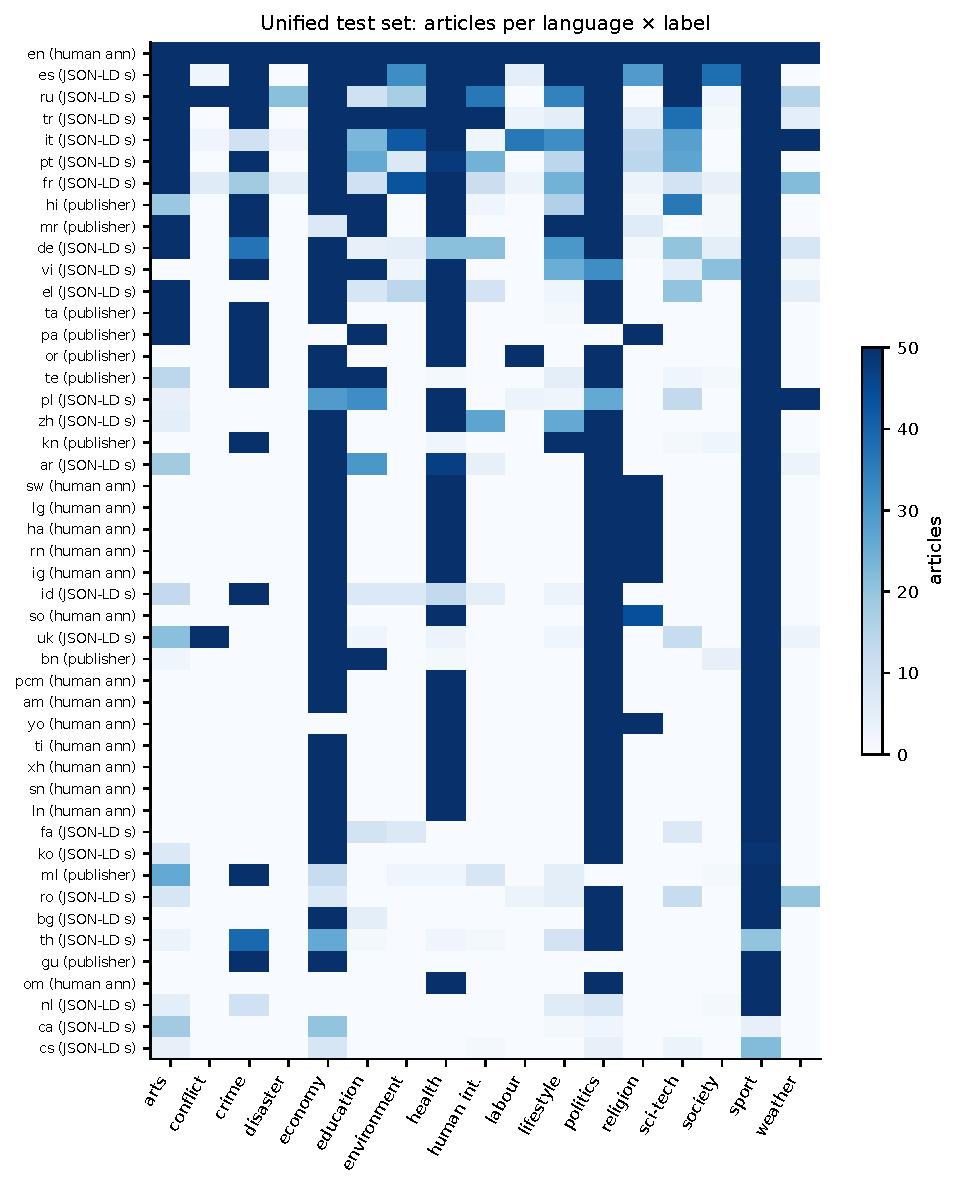
\includegraphics[width=\columnwidth]{figures/fig_testset_heatmap.pdf}
\caption{Articles in the unified test set per language and label (at most 50 per language--label pair). The label origin in brackets is the dominant one for that language.}
\label{fig:testset}
\end{figure}

\begin{figure}[!htbp]
\centering
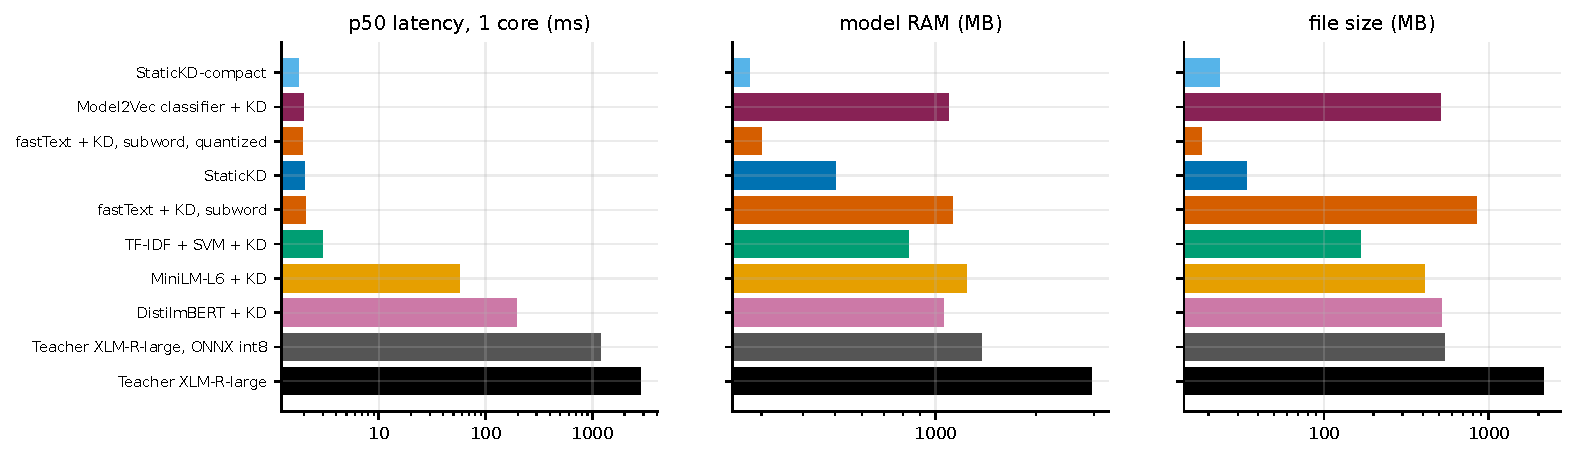
\includegraphics[width=0.9\textwidth]{figures/fig_latency_ram_size.pdf}
\caption{Latency per article, model RAM, and file size (log scale).}
\label{fig:latency}
\end{figure}

\begin{figure}[!htbp]
\centering
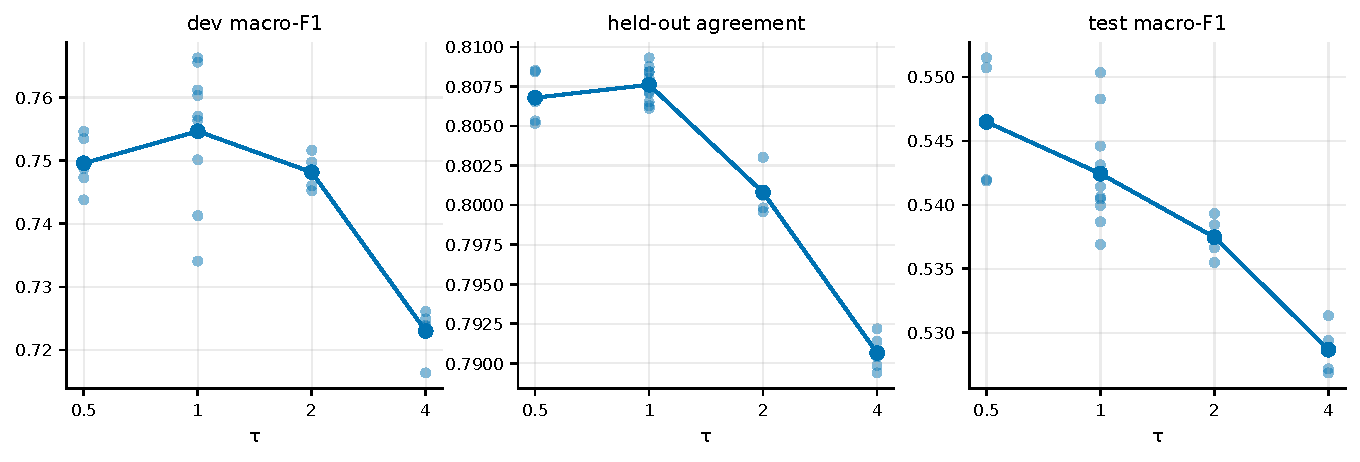
\includegraphics[width=0.9\textwidth]{figures/fig_temperature.pdf}
\caption{Effect of the distillation temperature. Each dot is one seed. The line connects the means.}
\label{fig:temperature}
\end{figure}

\begin{figure}[!htbp]
\centering
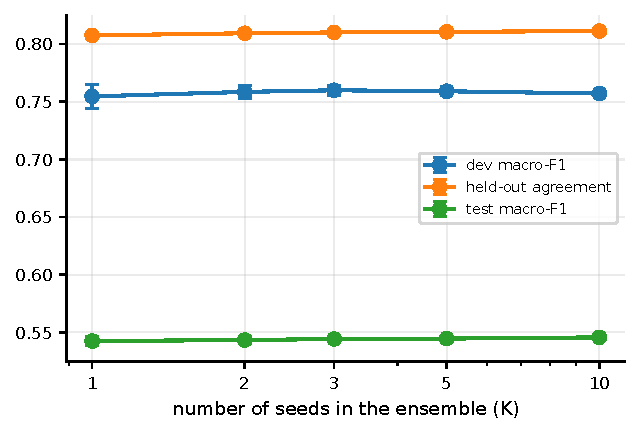
\includegraphics[width=0.85\columnwidth]{figures/fig_ensemble_size.pdf}
\caption{Effect of the table ensemble size (mean $\pm$ standard deviation over seed combinations).}
\label{fig:ensemble}
\end{figure}

\begin{figure}[!htbp]
\centering
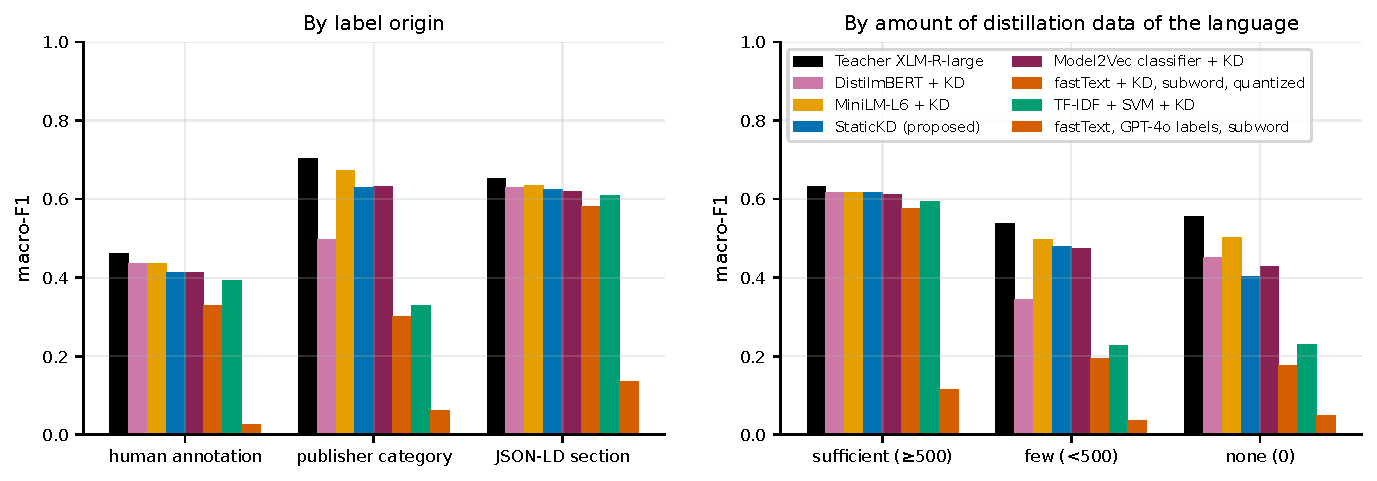
\includegraphics[width=0.78\textwidth]{figures/fig_groups.pdf}
\caption{Test macro-F1 by label origin (left) and by the amount of distillation data in the language of the article (right).}
\label{fig:groups}
\end{figure}

\begin{figure}[!htbp]
\centering
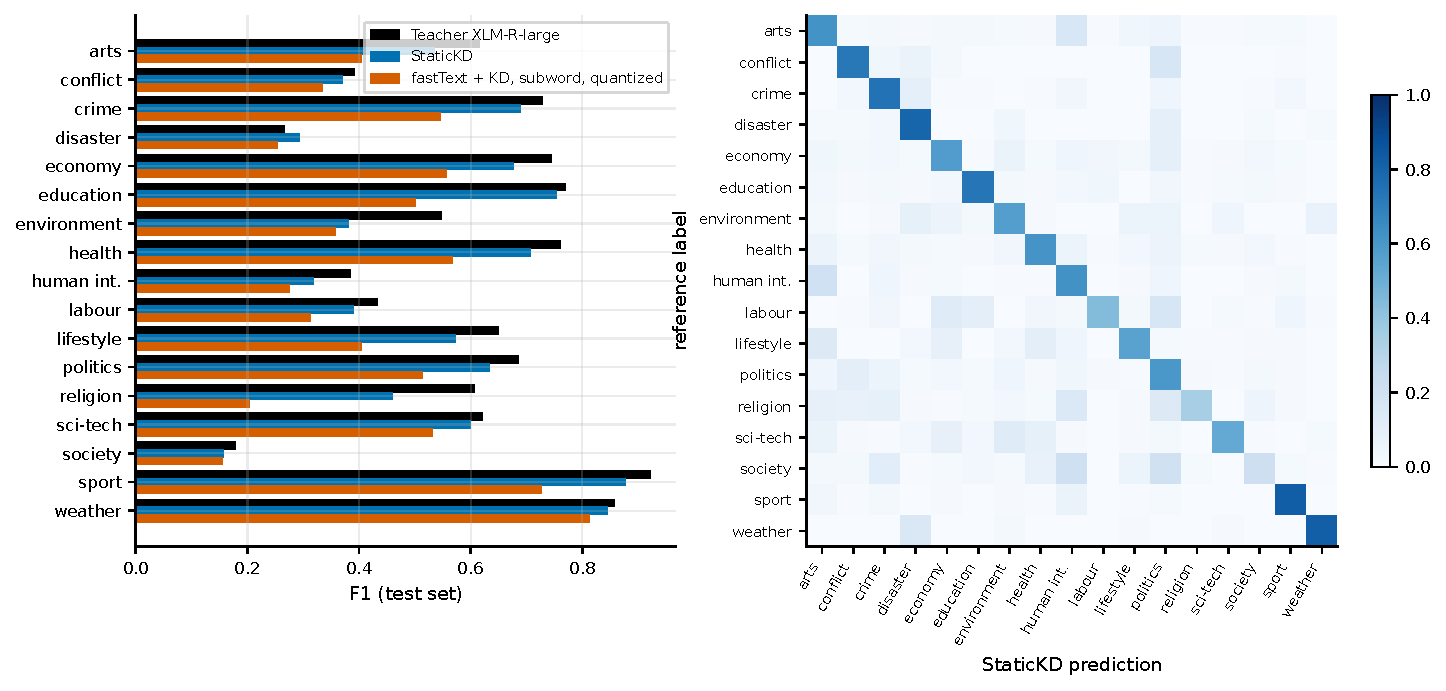
\includegraphics[width=0.9\textwidth]{figures/fig_per_label.pdf}
\caption{F1 per label on the test set (left) and the StaticKD confusion matrix normalized per reference label (right).}
\label{fig:label}
\end{figure}

\begin{figure}[!htbp]
\centering
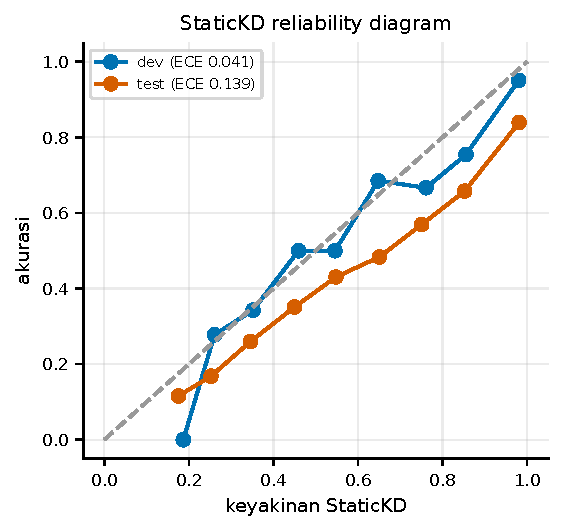
\includegraphics[width=0.8\columnwidth]{figures/fig_calibration.pdf}
\caption{Reliability diagram of StaticKD on the development and test sets.}
\label{fig:calib}
\end{figure}

\clearpage
\bibliographystyle{IEEEtran}
\bibliography{references}

\end{document}
